%++++++++++++++++++++++++++++++++++++++++
% Don't modify this section unless you know what you're doing!
\documentclass[letterpaper,12pt]{article}
\usepackage{tabularx} % extra features for tabular environment
\usepackage{amsmath}  % improve math presentation
\usepackage{graphicx} % takes care of graphic including machinery
\usepackage[margin=1in,letterpaper]{geometry} % decreases margins
\usepackage[final]{hyperref} % adds hyper links inside the generated pdf file
\hypersetup{
	colorlinks=true,       % false: boxed links; true: colored links
	linkcolor=blue,        % color of internal links
	citecolor=blue,        % color of links to bibliography
	filecolor=magenta,     % color of file links
	urlcolor=blue         
}
%++++++++++++++++++++++++++++++++++++++++

\usepackage{titling}
\pretitle{\begin{flushright}}
\posttitle{\par\end{flushright}}
\preauthor{\begin{flushright}}
\postauthor{\par\end{flushright}}
\predate{\begin{flushright}}
\postdate{\par\end{flushright}}

\usepackage[font=small,skip=0pt]{caption}

% \usepackage[demo]{graphicx}
\usepackage{subcaption}
\usepackage{float}

\usepackage{booktabs}

\usepackage[style=ieee,backend=biber]{biblatex}
\addbibresource{report.bib}

\begin{document}

\title{\vspace{-2cm} Kavi Dey}
\author{\vspace{-0.4cm} E157 RF Design \\ Lab Partner: Zoe Worrall \\ Design Project 2}
\date{\vspace{-0.4cm} \today}
\maketitle

% modified from https://www.overleaf.com/latex/templates/sample-lab-report-for-u-of-r-phys-349/pgsyqngcyjxk
%++++++++++++++++++++++++++++++++++++++++

% abstract
% \begin{abstract}
% abstract here
% \end{abstract}

% sections
\section{Summary Information}
The secret message is ``HMC''. The maximum range that we predicted our receiver would work at was 250 m.
The maximum range we were able to test was 72.3 m due to running out of cable length in the hallway.
The analytical system temperature was 8.22E+10 K and the measured temperature was 7.13E+07 K.
The analytical receiver IIP3 was -26.77 dBm and the measured one was -62.5 dBm.

\newpage
\section{Pictures of Received Data}
\begin{figure}[H]
	\begin{centering}
		\includegraphics[width=0.5\columnwidth,angle=-90]{figures/3m.img}
		\caption{Picture of setup at 3 m range}
	\end{centering}
\end{figure}

\begin{figure}[H]
	\begin{centering}
		\includegraphics[width=0.8\columnwidth]{figures/3m.trace}
		\caption{Oscilloscope trace at 3 m range}
	\end{centering}
\end{figure}

\begin{figure}[H]
	\begin{centering}
		\includegraphics[width=0.5\columnwidth]{figures/3m.spectra}
		\caption{Spectrum at 3 m range}
	\end{centering}
\end{figure}

\begin{figure}[H]
	\begin{centering}
		\includegraphics[width=0.5\columnwidth,angle=-90]{figures/maxm.img}
		\caption{Picture of setup at max range}
	\end{centering}
\end{figure}

\begin{figure}[H]
	\begin{centering}
		\includegraphics[width=0.8\columnwidth]{figures/maxm.trace}
		\caption{Oscilloscope trace at max range}
	\end{centering}
\end{figure}

\begin{figure}[H]
	\begin{centering}
		\includegraphics[width=0.5\columnwidth]{figures/maxm.spectra}
		\caption{Spectrum at max range}
	\end{centering}
\end{figure}


\newpage
\section{Oscilloscope Trace Decoding}
\begin{figure}[H]
	\begin{centering}
		\includegraphics[width=1.1\columnwidth]{figures/decoding.pdf}
		\caption{Annotated oscilloscope trace for decoding}
	\end{centering}
\end{figure}

The oscilloscope trace can be decoded by treating it as a 10 kbps signal where the high and low levels indicated above represents 1s and 0s respectively (the exact high level voltage depends on distance). The component representing the 0 frequency is attenuated by the mixer, so it is not visible and only the component representing the 1 frequency is left. The data is transmitted at 10 kbps so the duration of each bit is 0.1 ms.
\\
\\
\noindent
Each message starts with a \texttt{01010101} frame which can be ignored, followed by 24 bits encoded as described above. The 24 bits should be split up into groups of 8 and decoded as ASCII characters, resulting in the message ``HMC''.

\newpage
\section{Antenna Information}
\begin{figure}[H]
	\begin{centering}
		\includegraphics[width=0.8\columnwidth]{figures/antenna_anechoic.png}
		\caption{Hawking H-A16SD Antenna in anechoic chamber}
	\end{centering}
\end{figure}

As this is not an antenna we measured in lab 5, we extracted the radiation pattern and S11. The radiation pattern was measured in the RF lab anechoic chamber with the Keysight 8753D VNA on a turn table as pictured above. S21 was measured at incremental angles and the antenna gain was calculated using the following equation:
$$
G_{TX}=S21-G_{cal}-20\log\left(\frac{\lambda}{4\pi r}\right)
$$
Producing the following plot:
\begin{figure}[H]
	\begin{centering}
		\includegraphics[width=0.5\columnwidth]{figures/antenna.radiation}
		\caption{H-A16SD radiation pattern}
	\end{centering}
\end{figure}
\noindent
The directivity of this antenna is 3.49 dB. At 0 deg we also measured S11 and other S parameters:
\begin{figure}[H]
	\begin{centering}
		\includegraphics[width=0.7\columnwidth]{figures/antenna.sparams}
		\caption{H-A16SD S parameters}
	\end{centering}
\end{figure}
\noindent
At the frequency we are working at (around 2276 MHz) we measured an S11 of 0.39 dB which should be impossible for a passive component like an antenna. We hypothesize that this is due to our reference plane being too far away from the antenna and that the homemade RP-SMA to SMA adapter could be causing issues, but did not have time to test this.

\newpage
\section{Receiver Schematic}
\begin{figure}[H]
	\begin{centering}
		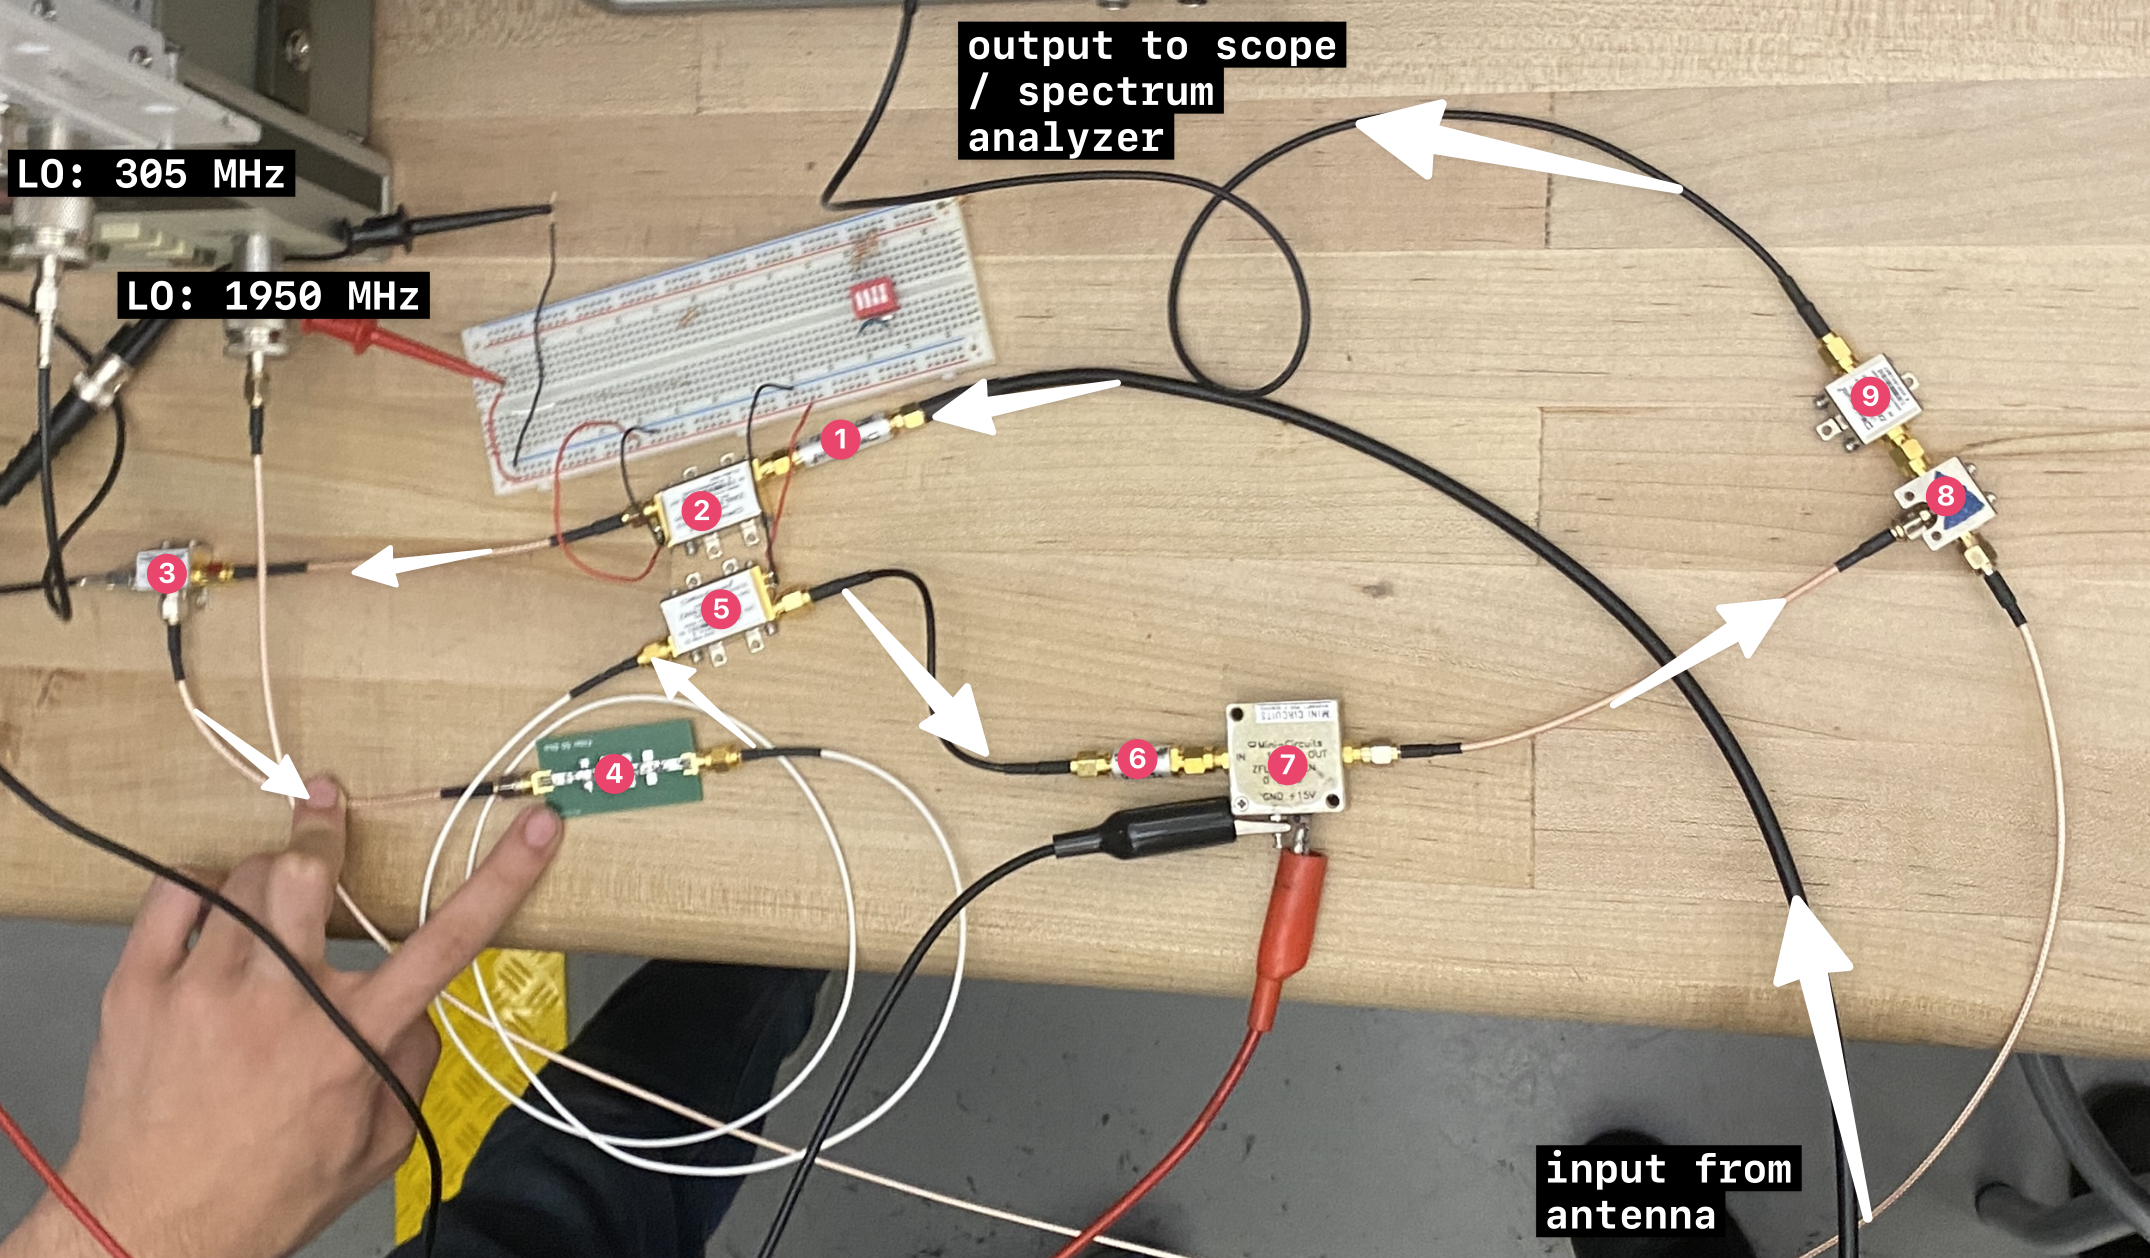
\includegraphics[width=1\columnwidth]{figures/receiver_picture.png}
		\caption{Picture of Receiver}
	\end{centering}
\end{figure}

\begin{figure}[H]
	\begin{centering}
		\includegraphics[width=1\columnwidth]{figures/receiver_schematic.pdf}
		\caption{Receiver Schematic}
	\end{centering}
\end{figure}

The custom bandpass filter was built as a 2nd order chebyshev filter designed using \href{https://markimicrowave.com/technical-resources/tools/lc-filter-design-tool/}{Marki LC Filter Design Tool}. The S21 log magnitude is provided below for reference
\begin{figure}[H]
	\begin{centering}
		\includegraphics[width=1\columnwidth]{figures/bpf_s21.png}
		\caption{Custom Bandpass filter S21}
	\end{centering}
\end{figure}

\newpage
\section{Receiver Spectra}
\begin{figure}[H]
	\begin{centering}
		\includegraphics[width=0.5\columnwidth]{figures/receiver_spectra/0.beginning}
		\caption{Stage 0: Raw antenna spectra}
	\end{centering}
\end{figure}
\noindent
Due to the high noise floor, it is not possible to see any peaks in this data.
\begin{figure}[H]
	\begin{centering}
		\includegraphics[width=0.5\columnwidth]{figures/receiver_spectra/1.bpf}
		\caption{Stage 1: After wide bandpass filter}
	\end{centering}
\end{figure}
\noindent
Due to the high noise floor, it is not possible to see any peaks in this data.
\begin{figure}[H]
	\begin{centering}
		\includegraphics[width=0.5\columnwidth]{figures/receiver_spectra/2.amp}
		\caption{Stage 2: After amplifier}
	\end{centering}
\end{figure}
\noindent
The two peaks at 2.258 and 2.298 GHz are the two tones of our signal. The peaks between 2.4 and 2.5 GHz are from WiFi, the small bump around 2.15 GHz is likely a cellular band using OFDM modulation.

\begin{figure}[H]
	\begin{subfigure}[t]{.49\textwidth}
		\centering
		\includegraphics[width=\linewidth]{figures/receiver_spectra/3.mixer.lower}
		\caption{IF Spectra}
	  \end{subfigure}
	  \hfill
	  \begin{subfigure}[t]{.49\textwidth}
		\centering
		\includegraphics[width=\linewidth]{figures/receiver_spectra/3.mixer.upper}
		\caption{RF Spectra}
	  \end{subfigure}

	  \vspace{0.5cm}
	  \caption{Stage 3: After mixer (LO = 1950 MHz)}
\end{figure}
\noindent
In the IF spectra the peaks at 311.3 and 347.1 MHz are the two tones of our signal. The peaks from 450 Mhz to 485 MHz are from WiFi as before, and the bump around 100 MHz is cellular signal. There are no peaks in the RF spectra because the low input power to the mixer was not enough to cause leakage above the noise floor.
\begin{figure}[H]
	\begin{centering}
		\includegraphics[width=0.5\columnwidth]{figures/receiver_spectra/4.bpf}
		\caption{Stage 4: After bandpass filter}
	\end{centering}
\end{figure}
\noindent
The peaks at 311.3 and 347.1 MHz are the two tones of our signal. A small peak from WiFi that was not fully filtered out is visible around 460 MHz.

\begin{figure}[H]
	\begin{centering}
		\includegraphics[width=0.5\columnwidth]{figures/receiver_spectra/5.amp}
		\caption{Stage 5: After amplifier}
	\end{centering}
\end{figure}
\noindent
In the IF spectra the peaks at 311.3 and 347.1 MHz are the two tones of our signal. The peaks from 450 to 500 MHz are from WiFi. The shape of the noise floor has changed due to the bandpass filter.

\begin{figure}[H]
	\begin{centering}
		\includegraphics[width=0.5\columnwidth]{figures/receiver_spectra/6.attenuator}
		\caption{Stage 6: After attenuator}
	\end{centering}
\end{figure}
\noindent
The peaks visible after the attenuator are the same as before the attenuator, just decreased by 3 dB.

\begin{figure}[H]
	\begin{centering}
		\includegraphics[width=0.5\columnwidth]{figures/receiver_spectra/7.amp}
		\caption{Stage 7: After amplifier}
	\end{centering}
\end{figure}
\noindent
The peaks at 311.3 and 347.1 MHz are the two tones of our signal. The bump at 380 MHz is due to the shape of the bandpass filter. The peaks between 450 and 500 MHZ are from WiFi. Note that the amplifier added additional noise around 100 MHz.

\begin{figure}[H]
	\begin{subfigure}[t]{.49\textwidth}
		\centering
		\includegraphics[width=\linewidth]{figures/receiver_spectra/8.mixer.lower}
		\caption{IF Spectra}
	  \end{subfigure}
	  \hfill
	  \begin{subfigure}[t]{.49\textwidth}
		\centering
		\includegraphics[width=\linewidth]{figures/receiver_spectra/8.mixer.upper}
		\caption{RF Spectra}
	  \end{subfigure}

	  \vspace{0.5cm}
	  \caption{Stage 8: After mixer}
\end{figure}
In the IF spectra the peaks at 6.4 and 42 MHz are the two tones of our signal. The bump around 80 MHz is due to the shape of the bandpass filter. The peaks in the RF spectra are leakage through the mixer due to the higher power. They appear at similar frequencies as to before the mixer.

\begin{figure}[H]
	\begin{subfigure}[t]{.49\textwidth}
		\centering
		\includegraphics[width=\linewidth]{figures/receiver_spectra/9.lpf.lower}
		\caption{IF Spectra}
	  \end{subfigure}
	  \hfill
	  \begin{subfigure}[t]{.49\textwidth}
		\centering
		\includegraphics[width=\linewidth]{figures/receiver_spectra/9.lpf.upper}
		\caption{RF Spectra}
	  \end{subfigure}

	  \vspace{0.5cm}
	  \caption{Stage 9: After lowpass filter}
\end{figure}
In the IF spectra the peaks at 6.4 and 42 MHz are the two tones of our signal. There are no peaks in the RF spectra as the lowpass filter has filtered them out.

\newpage
\section{Theoretical Signal and Noise Levels} \label{sec:sig_and_noise}
The link and noise budget excel spreadsheet with all calculations is here \url{github.com/kavidey/e157/raw/refs/heads/main/dp_02/receiver/link_budget.xlsx}
\subsection{Signal Level Theory}
Signal levels were calculated at each component in the receiver chain using their corresponding equations. Passive components including mixers, filters, and attenuators reduce signal strength via insertion loss. Amplifiers increase signal strength via gain, and generate distortion and intermodulation harmonics. For this report, we only focused on the IM3 harmonics those are in the baseband and we are not doing direct downconversion. IM3 harmonic size was calculated from OIP3 and IIP3 using the following formula:
$$
IM3 = OIP3 - 3 \cdot (IIP3 - Pin)
$$
OIP3 was read off of amplifier datasheets directly (\href{https://www.mouser.com/datasheet/2/1030/ZX60-2531MA_2b-1701661.pdf}{ZX60-2531MA+} and \href{https://www.mouser.com/datasheet/2/1030/ZFL_1000LN_2b-2303490.pdf}{ZFL-1000LN}). IIP3 was calculated from datasheet ``Output power at P-1dB'' as $IIP3 = P_{-1dB,out} - (G_{ain} - 1) + 9.6$. Propagating power through each step of the receiver chain. A full list of important component properties in section \ref{sec:additional}.
\begin{figure}[H]
	\begin{centering}
		\includegraphics[width=1\columnwidth]{figures/signal_theory}
		\caption{Theoretical and measured signal power levels}
	\end{centering}
\end{figure}
\noindent
These calculations were repeated for 3 m and max range test which are available in the spreadsheet linked above. In all cases the predicted noise power is quite a bit higher than the measured one. In the example above, the predicted baseband power is much larger than the expected, resulting in massively larger IM3 components.
\subsection{Noise Level Theory}
Noise levels were calculated in a few steps. First, the noise temperature of each component was calculated from theory: $T_p = \left(\frac{1}{L}-1\right)T$ for passives and $T_a = (nf-1)T$ for amplifiers. Next, the system temperature at each point in the receive chain was calculated as $T_{out} = \{G \text{ or } L \} \cdot(T_{in} + T_d)$ where $T_d$ is the component temperature. Notably the system temperature was multiplied by two for mixers as the produce two copies of the noise. This temperature was also converted to dBm for easier comparison to measured noise level. Note that the assumed antenna noise as 290K from pointing at earth.
\begin{figure}[H]
	\begin{centering}
		\includegraphics[width=1\columnwidth]{figures/noise_theory}
		\caption{Theoretical and measured signal noise levels}
	\end{centering}
\end{figure}
\noindent
Similar to the signal power, the analytical noise temperature much larger (three orders of magnitude higher) than the measured noise temperature. Both of these is likely due to over estimating the gain of the amplifiers.
\\
\\
\noindent
The theoretical maximum range was calculated by testing different distances in the spreadsheet until the signal power was equal to the noise power.

\newpage
\section{IP3 Distortion Characterization}
To measure the IIP3 of our amplifier we replaced the antenna with a two tone signal generator. We tested a range of input powers and measured the output power of the fundamental and the IM3 terms to make the following plot.
\begin{figure}[H]
	\begin{centering}
		\includegraphics[width=0.7\columnwidth]{figures/iip3_regression.pdf}
		\caption{Analytical and measured IIP3}
	\end{centering}
\end{figure}
Running a linear regression we get:
\\
\begin{center}
	\begin{tabular}{lrr}
		\toprule
		Term & Slope & Intercept \\
		\midrule
		Linear & 1.21 & 30.12 \\
		3rd Order & 2.9 & 75.34 \\
		\bottomrule
	\end{tabular}
\end{center}

\noindent
To calculate the analytical IP3 point we used the following logic. We only need to consider the IM3 components generated by the last amplifier because they are orders of magnitude larger than the earlier ones. This allows us to simplify the receiver chain into gain $\to$ amplifier $\to$ attenuation.
\\
\\
\noindent
Adding additional (assumed perfectly linear) gain $G$ before the final amplifier reduces the input power needed to achieve the same output power. In other words reduces $IIP3$ to $IIP3_{combined} = IIP3_{amplifier} - G$ while keeping the same $OIP3$. Adding additional attenuation $L$ after the final amplifier reduces the total output, keeping $IIP3$ the same and reducing $OIP3$ to $OIP3_{combined} = OIP3_{amplifier} - L$.
\\
\\
\noindent
Our final amplifier (stage 7) is the ZFL-1000LN which has an $IIP3$ of -6.4 dBm and $OIP3$ of 14 dBm (from the \href{https://www.mouser.com/datasheet/2/1030/ZFL_1000LN_2b-2303490.pdf}{device datasheet}). Adding up all the amplification and attenuation from stages 1-6, we get $G$ = 56.1 dBm and addding up the attenuation from stages 8-9 we get $L$ = -7 dBm. This results in analytical $IIP3$ = -62.5 and $OIP3$ = 7 dBm.
\\
\\
\noindent
To verify this calculation, we tested different power values in the signal and noise level excel spreadsheet we made for section \ref{sec:sig_and_noise} until the IM3 components were equal to the signal power. This yielded an $IIP3$ = -61 dBm and $OIP3$ = 10 dBm, fairly close to the other analytical method.
\\
\\
\noindent
Note that both analytical methods are fairly far away from the measured value. This is likely due to a combination of noisy measurements (neither line in the measured plot has the correct slope) and incorrect gain/IIP3/OIP3 values as discussed in section \ref{sec:sig_and_noise}. The data here implies that IIP3 and gain before stage 7 are less accurate the OIP3 and the attenuation after stage 7.
% Pout vs. Pin plot showing fundamental power and IM3 power at the output of your receiver in the receiver characterization test configuration.
% Extrapolate measured lines to indicate a measured IP3.
% Include a point showing your theoretical IP3.
% Include a calculation below (with references to datasheets where appropriate) to explain how you calculated your theoretical IP3.

% \newpage
% \section{Discussions \label{sec:discussion}}
% Discussion of discrepancies between analytical, simulated and measured results.  Quantitatively justify differences between them, including any modifications you made to your models to make your simulations match your measurements better (e.g.: board parasitics).  Refer to prior figures in your report for supporting evidence in this discussion.

\newpage
\section{Additional Notes} \label{sec:additional}
All of the data, code, and figures are available in this github repo: \url{github.com/kavidey/e157/tree/main/dp_02}. 

\begin{figure}[H]
	\begin{centering}
		\includegraphics[width=1\columnwidth]{figures/params}
		\caption{Receiver component parameters (from datasheets and calculated)}
	\end{centering}
\end{figure}

% \begin{enumerate}
%   \item \texttt{schematics/} has the pretty display schematics made in Altium
% \end{enumerate}

% \newpage
% \section{Takeaways}
% One paragraph about one thing you learned about RF design doing this project.

% \newpage
% \section{Bibliography}
% \printbibliography

% referencing bibliography
% ~\cite{melissinos, Cyr, Wiki}

% figures
% \begin{figure}[ht] 
%     \centering \includegraphics[width=0.8\columnwidth]{sr_setup}
%     \caption{
%             \label{fig:samplesetup}
%             Every figure MUST have a caption.
%     }
% \end{figure}

% equations
% \begin{equation} \label{eq:aperp} % the label is used to reference the equation
%     u(\lambda,T)=\frac{8\pi hc\lambda^{-5}}{e^{hc/\lambda kT}-1},
% \end{equation}
%
% ~\ref{fig:samplesetup}

% tables
% \begin{table}[ht]
%     \begin{center}
%         \caption{Every table needs a caption.}
%         \label{tbl:bins} % spaces are big no-no withing labels
%         \begin{tabular}{|cc|}
%             \hline
%             \multicolumn{1}{|c}{$x$ (m)} & \multicolumn{1}{c|}{$V$ (V)} \\
%             \hline
%             0.0044151                    & 0.0030871                    \\
%             0.0021633                    & 0.0021343                    \\
%             0.0003600                    & 0.0018642                    \\
%             0.0023831                    & 0.0013287                    \\
%             \hline
%         \end{tabular}
%     \end{center}
% \end{table}
%
% Table~\ref{tbl:bins} is an example.

% \newpage

% bibliography
% \begin{thebibliography}{99}
%     \bibitem{levitator_paper}
%     Asier Marzo, Adrian Barnes, Bruce W. Drinkwater; TinyLev: A multi-emitter single-axis acoustic levitator. \textit{Rev. Sci. Instrum.} 1 August 2017; 88 (8): 085105. \href{https://doi.org/10.1063/1.4989995}{https://doi.org/10.1063/1.4989995}

%     \bibitem{levitator_instructions}
%     Instructables ultrasonic levitator materials and instructions. \href{https://www.instructables.com/Acoustic-Levitator/}{https://www.instructables.com/Acoustic-Levitator/}
% \end{thebibliography}
\end{document}